\title{Unoffical notes: Search for boosted top+Higgs resonance in the all hadronic decay mode}
\author{Lucas Corcodilos}
\date{\today}

\documentclass[10pt,oneside]{article}
\usepackage[margin=0.75in]{geometry}
\usepackage{graphicx}
\usepackage{url}
\usepackage{float}
\usepackage{makecell}
\usepackage{hyperref}
\hypersetup{
    colorlinks,
    citecolor=black,
    filecolor=black,
    linkcolor=black,
    urlcolor=black
}
\restylefloat{table}

\begin{document}
\maketitle
\tableofcontents
\section{Analysis strategy and selection}

Dijet search for boosted $X \to tH$. The benchmark, $X$, is a VLQ $T'$ produced
in association with a bottom quark. The interaction with an associated top quark
is currently ignored since the simulation samples are inconsistent with the UL
versions available for all other simulation. The associated quark will have 
much lower transverse momentum than the T' decay products and so the affect on
the analysis is expected to be small (ie. quark will be along beamline).

\subsection{Selection}
\begin{table}[H]
    \centering
    \begin{tabular}{|c |c |c |c|}
        \hline
        Signal region (SR) & QCD control for SR & Validation region (VR) & QCD control for VR \\
        \hline
        \multicolumn{4}{|c|}{Two AK8 jets separated by $\Delta \phi > \pi/2$} \\
        \multicolumn{4}{|c|}{$p_T > 350$ GeV for each jet} \\
        \multicolumn{4}{|c|}{$|\eta| < 2.4$ for each jet} \\
        \multicolumn{4}{|c|}{$m_{\mathrm{jet}} > 50$ for each jet} \\
        \hline
        \multicolumn{2}{|c|}{At least one jet top tagged} & \multicolumn{2}{|c|}{No jet top tagged} \\
        \hline
        \multicolumn{1}{|c|}{Higgs tag pass} & \multicolumn{1}{|c|}{Higgs tag fail} & \multicolumn{1}{|c|}{Higgs tag pass} & \multicolumn{1}{|c|}{Higgs tag fail} \\
        \hline
    \end{tabular} 
    \caption{Analysis selection for four selection regions. The definitions of the ``top tag'' and ``Higgs tag'' can be
    found in \ref{table:tags}.}
    \label{table:selection}
\end{table}

\begin{table}[H]
    \centering
    \begin{tabular}{c c c c}
         & DeepAK8 & Particle Net & Mass \\
        \hline
        Top quark & 0.94 & 0.94 & [105,210] GeV \\
        Higgs boson & \makecell{0.96\\(mass-decorrelated)} & \makecell{0.98\\(mass-decorrelated)} & - \\
    \end{tabular} 
    \caption{Selections for top and Higgs jet tagging. The analysis considers using either DeepAK8 or ParticleNet so
    the working points for both are provided. Note that the Higgs tag uses the mass-decorrelated version of each tagger
    and does not use a jet mass selection because of the nature of the background estimate. The choice of NN-scores
    is based off of $S/\sqrt{B}$ optimization of the four different variables with N-1 cuts, as shown in Figs.\ref{figs:jetDAK8} and \ref{figs:jetPN}.}
    \label{table:tags}
\end{table}


\section{Initial studies on jet tagging}
\label{sec:jets}
Two neural network based taggers are considered for jet tagging -
DeepAK8 and ParticleNet. Several aspects of these taggers can affect this
analysis and are considered when choosing between the taggers.

First and most importantly, the tagger must be decorrelated from the jet
mass so as not to sculpt the jet mass distribution. The two dimensional background
estimation method uses the jet mass as one of the axis in which to measure data.
If the taggers sculpt the jet mass so as to create a signal-like peak, the background
will be harder to discriminant from potential signal.

Additionally, the data-driven
estimate of the QCD multijet background relies on a smooth ratio of the distributions
of those events passing and failing the tagger. If the ``pass'' is sculpted and the ``fail''
is not, we cannot hope to use our transfer function method without introducing method
for potential signal bias.

Second, the tagger should be good at distinguishing between top and Higgs jets so the
tagger can be used to easily identify which side of the event is which physics object.
In particular, the analysis would benefit from a tagger that correctly identifes that 
real Higgs jets are not top jets.

Finally, the tagger should be efficient at removing background without requiring a 
MC-to-data scale factor that is large or has large uncertainties that could dominant
the total systematic uncertainty for the analysis.

With these three items in mind, we examined two variables - the difference in mass
between the two jets and the difference in top tagging scores between the two jets
- and plotted them against each other. In addition to considering the two taggers,
we also considered four scenarios based on the simulation truth.

From left to right in Figs. \ref{figs:DeepAK8_diff_2D} and \ref{figs:PN_diff_2D}:
\begin{itemize}
    \item The first scenario does nothing with simulation truth.
    \item The second scenario examines when neither the top nor Higgs jet identified by the
          tagger were able to be matched to their respective generator particle (``Bad match'').
    \item The third scenario examines when both the top and Higgs jets identified by the tagger
          were matched successfully to their respective generator particle (``Good match'').
    \item The fourth scenario identifies the top and Higgs jets based on the generator particle
          information and then the variables plotted are calculated based on this information.
\end{itemize}

In other words, the fourth scenario flips the order of operations of the third scenario.
The distributions for both taggers and the four scenarios are shown in Figs.
\ref{figs:DeepAK8_diff_2D} and \ref{figs:PN_diff_2D} where a 2016 $T' \to tH$ signal with
a $T'$ mass of 1200 GeV is examined.

\begin{figure}[H]
    \centering
    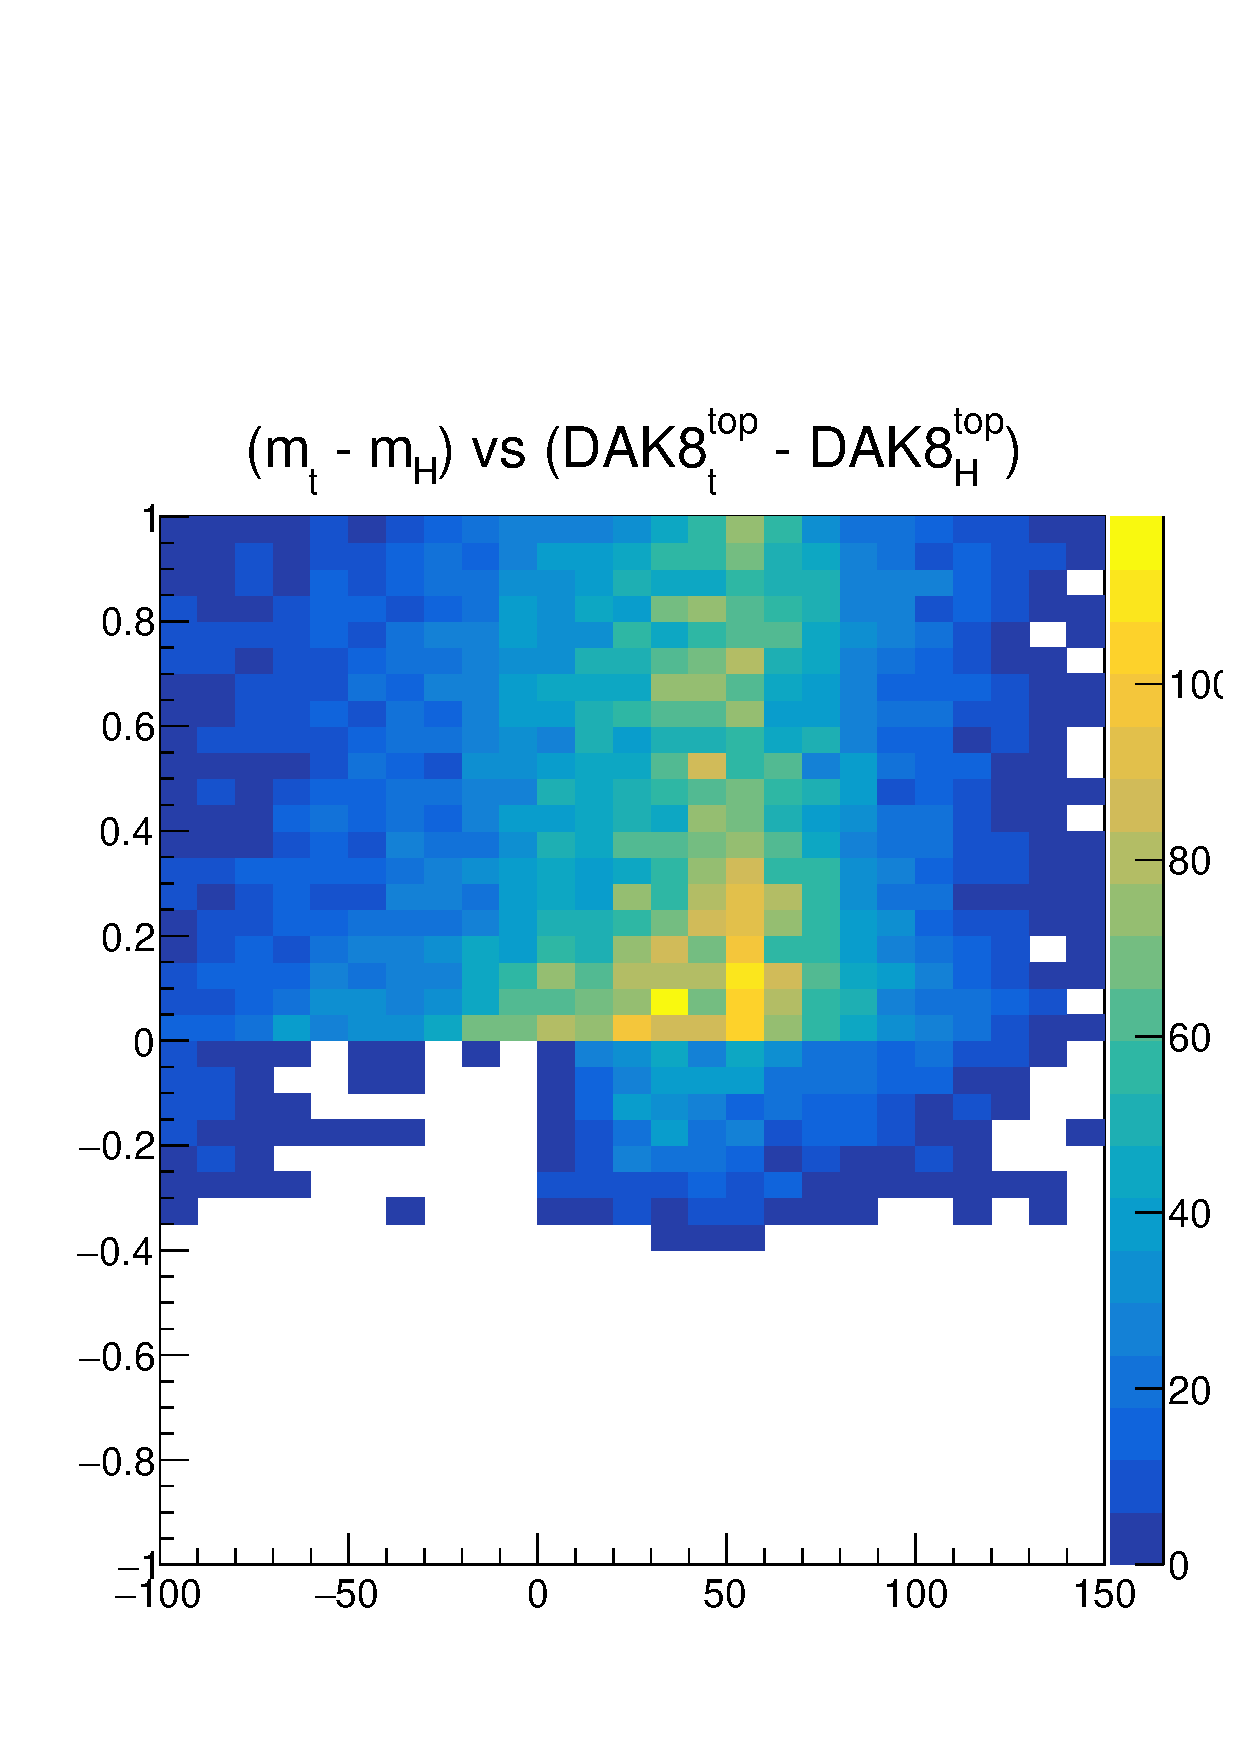
\includegraphics[page=1,width=0.24\textwidth]{../plots/diff2Dstudy.pdf}
    \includegraphics[page=2,width=0.24\textwidth]{../plots/diff2Dstudy.pdf}
    \includegraphics[page=3,width=0.24\textwidth]{../plots/diff2Dstudy.pdf}
    \includegraphics[page=4,width=0.24\textwidth]{../plots/diff2Dstudy.pdf}
    \caption{DeepAK8 studies}
    \label{figs:DeepAK8_diff_2D}
\end{figure}

\begin{figure}[H]
    \centering
    \includegraphics[page=5,width=0.24\textwidth]{../plots/diff2Dstudy.pdf}
    \includegraphics[page=6,width=0.24\textwidth]{../plots/diff2Dstudy.pdf}
    \includegraphics[page=7,width=0.24\textwidth]{../plots/diff2Dstudy.pdf}
    \includegraphics[page=8,width=0.24\textwidth]{../plots/diff2Dstudy.pdf}
    \caption{ParticleNet studies}
    \label{figs:PN_diff_2D}
\end{figure}


\section{Kinematic distributions}

% We further investigate kinematic variables which may be useful in increasing
% the signal to background ratio in the analysis. Figures \ref{figs:pt} and 
% \ref{figs:etaY} compare simulation for all of Run 2.

\begin{figure}[H]
    \includegraphics[width=0.32\textwidth]{../plots/pt0_Run2.pdf}
    \includegraphics[width=0.32\textwidth]{../plots/pt1_Run2.pdf}
    \includegraphics[width=0.32\textwidth]{../plots/HT_Run2.pdf}
    \caption{The $p_T$ of the leading (left) and subleading (middle) jet in the event and the scalar sum of the two (right).
    The total background is represented as a stack of QCD (yellow) and ttbar (red) MC and the total is normalized to
    unity. The signal (black line) is separately normalized to unity.}
    \label{figs:pt}
\end{figure}

% \begin{figure}[H]
%     \includegraphics[width=0.49\textwidth]{../plots/deltaEta_Run2.pdf}
%     \includegraphics[width=0.49\textwidth]{../plots/deltaY_Run2.pdf}
%     \caption{The $|\Delta \eta|$ between the two candidate jets in the event. The total background
%     is represented as a stack of QCD (yellow) and ttbar (red) MC and the total is normalized to
%     unity. The signal (black line) is separately normalized to unity.}
%     \label{figs:etaY}
% \end{figure}


\section{Jet tagging variables}

Two variables are used to tag a canidate jet - the tagger score and the jet mass.
In order to inspect these variables, a series of N-1 plots are made - one for each
the top jet mass, top jet tagger score, Higgs jet mass, and Higgs jet tagger score.
When one variable is plotted, the other three are cut on.

Since this means a Higgs and top cannot be identified without impacting the distributions,
the top quark is assumed to be the leading jet in $p_T$. The MC truth shows this is true 50\%
of the time. The other N-1 cuts in a given plot should kill most
of the mis-matched events (where the top jet is actually a Higgs and vice versa)
with some fraction remaining. As can be seen in \ref{figs:DeepAK8_diff_2D}, that 
fraction is decently large when tagging a
real Higgs with the DeepAK8 top tagger. This effect explains the Higgs peak
in Figure \ref{figs:jetMassDAK8}.

Figures \ref{figs:jetMassDAK8}, \ref{figs:jetMassPN}, \ref{figs:jetDAK8}, and \ref{figs:jetPN}
compare simulation for all of Run 2.

\begin{figure}[H]
    \includegraphics[width=0.49\textwidth]{../plots/optimization/mH_deepTag_cut_nminus1_Run2.pdf}
    \includegraphics[width=0.49\textwidth]{../plots/optimization/mt_deepTag_cut_nminus1_Run2.pdf}
    \caption{Shape comparison of the jet mass distributions for the Higgs (left) and top (right) jets
    when using the mass decorrelated DeepAK8 tagger. The total background
    is represented as a stack of QCD (yellow) and ttbar (red) MC and the total is normalized to
    the expected number of background events. The signal (black line) is separately normalized to the expected
    number of signal events assuming the cross section is 1pb.}
    \label{figs:jetMassDAK8}
\end{figure}

\begin{figure}[H]
    \includegraphics[width=0.49\textwidth]{../plots/optimization/mH_particleNet_cut_nminus1_Run2.pdf}
    \includegraphics[width=0.49\textwidth]{../plots/optimization/mt_particleNet_cut_nminus1_Run2.pdf}
    \caption{Shape comparison of the jet mass distributions for the Higgs (left) and top (right) jets
    when using the ParticleNet tagger (not mass decorrelated). The total background
    is represented as a stack of QCD (yellow) and ttbar (red) MC and the total is normalized to
    the expected number of background events. The signal (black line) is separately normalized to the expected
    number of signal events assuming the cross section is 1pb.}
    \label{figs:jetMassPN}
\end{figure}

\begin{figure}[H]
    \includegraphics[width=0.49\textwidth]{../plots/optimization/deepTag_H_cut_nminus1_Run2.pdf}
    \includegraphics[width=0.49\textwidth]{../plots/optimization/deepTag_top_cut_nminus1_Run2.pdf}
    \caption{Shape comparison of the DeepAK8 score distributions for the Higgs (left) and top (right) jets
    when using the mass decorrelated DeepAK8 tagger. The total background
    is represented as a stack of QCD (yellow) and ttbar (red) MC and the total is normalized to
    the expected number of background events. The signal (black line) is separately normalized to the expected
    number of signal events assuming the cross section is 1pb.}
    \label{figs:jetDAK8}
\end{figure}

\begin{figure}[H]
    \includegraphics[width=0.49\textwidth]{../plots/optimization/particleNet_H_cut_nminus1_Run2.pdf}
    \includegraphics[width=0.49\textwidth]{../plots/optimization/particleNet_top_cut_nminus1_Run2.pdf}
    \caption{Shape comparison of the ParticleNet score distributions for the Higgs (left) and top (right) jets
    when using the mass decorrelated ParticleNet tagger. The total background
    is represented as a stack of QCD (yellow) and ttbar (red) MC and the total is normalized to
    the expected number of background events. The signal (black line) is separately normalized to the expected
    number of signal events assuming the cross section is 1pb.}
    \label{figs:jetPN}
\end{figure}

\section{Background estimation method}

This analysis uses the 2D Alphabet method to build a 2D binned likelihood model that simultanously fits
ttbar from MC templates while fitting QCD using a data-driven method. The data-driven method uses
events in a QCD control region defined by inverting the tagging score selection on the Higgs jet.
A two-dimensional polynomial called the pass-fail ratio ($R_{P/F}$) is used as the transfer function between this control region and the signal
region. Additionally, there is no cut placed on the Higgs jet mass and instead, the Higgs jet mass sidebands
are used to constrain the backgrounds as well as interpolate the value of the background through the Higgs
mass signal region while blinded.

This method has been used successfully in B2G-19-003 and B2G-20-004. However, those two analyses used the 
QCD MC to assist the fit. Specifically, the $R_{P/F}^{MC}$ is calculated in simulation smoothed by a Kernel Density Estimate (KDE)
and the fitted polynomial becomes the $R_{ratio}$. Then, $R_{P/F} = R_{P/F}^{MC} * R_{ratio}$. By doing this, the fitted function
is only responsible for fitting the difference between MC and data which is often a less complex shape, reducing the number of necessary
parameters and stabalizing the model.

The $R_{ratio}$ variation of 2D Alphabet is noted because this analysis \textit{does not} use it 
with the primary reason being a lack of QCD MC statistics. Figure~\ref{figs:QCDSR} shows the 
QCD yield predicted by QCD simulation after the different HT-binned samples have been combined (via proper
normalization to respective cross sections) and the three eras of 2016, 2017, and 2018 summed. The fluctuations from simulation statistics 
are large enough that even a smoothing algorithm would have a difficult time reconstructing a smooth distribution
that could still lead to meaningful information for the background model.

\begin{figure}
    \centering
    \includegraphics[page=1,width=0.40\textwidth]{../plots/QCD_shapes.pdf}
    \includegraphics[page=3,width=0.40\textwidth]{../plots/QCD_shapes.pdf}
    \caption{QCD MC simulation yields in ``pass'' selection for DeepAK8 (left) and ParticleNet (right). In the lower-right
    of each subfigured is the integrated yield (after stitching samples and normalizing to Run 2 luminosity). The legends
    in the upper-right show the total number of simulated events.}
    \label{figs:QCDSR}
\end{figure}

Finally, a similar issue is faced with the $t\bar{t}$ simulation. The number of raw events in the signal region
is larger than that of the QCD simulation but the distributions fluctuate enough that there were fit stability issues.
This was studied with different $R_{P/F}$ parameterizations and coarser binning schemes but results were unstable.
In particular, HESSE was unable to determine fit uncertainties because of ``on boundary'' parameters. This was true
across the various $R_{P/F}$ and binning attempts.

To remedy the situation, the $t\bar{t}$ selections were reperformed with a looser selection on the Hbb tagging score
(to 0.8 for DeepAK8 and ParticleNet) and the resulting distributions scaled to the integrated yield when using the optimized
tagger selection. The loose working point of 0.8 was chosen based on 
Figs.~\ref{figs:jetDAK8} and~\ref{figs:jetPN} which show that the $t\bar{t}$ simulation statistics can be roughly doubled
by increasing the selection window. Since the loosening of the Hbb score effectively migrates $t\bar{t}$ events from
our ``fail'' region to the ``pass'' region, the possibility of biasing the shape in the ``pass'' to look more like the
distribution in the ``fail'' is possible. However, the comparisons in Figs.~\ref{figs:ttbarScaleCompDAK8} and~\ref{figs:ttbarScaleCompPN}
of the $t\bar{t}$ in the case of the raw selection (left) and the above ``loose-and-scale'' algorithm (right) show that the ``fail''
distributions are very similar and the ``pass'' distribution does not appear to be biased to look more like the ``fail''.

To substantiate that the resulting fit is healthier with the ``loose-and-scale'' method, Figs.~\ref{figs:ttbarScaleNuisCompDAK8}
and~\ref{figs:ttbarScaleNuisCompPN} compare the nuisance parameter pulls for the DeepAK8 and ParticleNet scenarios, respectively.

Additionally, Figs.~\ref{figs:jetDAK8} and~\ref{figs:jetPN} show that loosening the Hbb score is more
effective than loosening the top tagging score since most of the $t\bar{t}$ already lives in the signal selection of
these top score distributions. Loosening the top tagging score to 0.8 was attempted and the above understanding was confirmed
with little change to the final simulation statistics being observed.

\begin{figure}[H]
    \centering
    \includegraphics[width=0.4\textwidth]{../plots/fit_results/dataTH1200Blind_ttraw_DAK8_v2_0x0/SR/plots/fit_b/ttbar_18_projx_fitb.pdf}
    \includegraphics[width=0.4\textwidth]{../plots/fit_results/dataTH1200Blind_ttscaled_DAK8_v2_0x0/SR/plots/fit_b/ttbar_scaled_18_projx_fitb.pdf}
    \caption{The $m_H$ mass distributions of the 2018 $t\bar{t}$ simulation for the blinded background-only fit using the DeepAK8 tagger and a 0x0 $R_{P/F}$.
    The black points and vertical bars represent the post-fit value and uncertainty. The red histogram and shaded region represent the pre-fit value and uncertainty.}
    \label{figs:ttbarScaleCompDAK8}
\end{figure}
\begin{figure}[H]
    \centering
    \includegraphics[width=0.48\textwidth]{../plots/fit_results/dataTH1200Blind_ttraw_DAK8_v2_0x0/nuisance_pulls.pdf}
    \includegraphics[width=0.48\textwidth]{../plots/fit_results/dataTH1200Blind_ttscaled_DAK8_v2_0x0/nuisance_pulls.pdf}
    \caption{The nuisance parameter pulls for the blinded fits of the DeepAK8 based selection using a 0x0 $R_{P/F}$ for the raw $t\bar{t}$ MC (left) and 
    $t\bar{t}$ MC with a looser selection and scaled down (right).}
    \label{figs:ttbarScaleNuisCompDAK8}
\end{figure}

\begin{figure}[H]
    \centering
    \includegraphics[width=0.4\textwidth]{../plots/fit_results/dataTH1200Blind_ttraw_PN_v2_0x0/SR/plots/fit_b/ttbar_18_projx_fitb.pdf}
    \includegraphics[width=0.4\textwidth]{../plots/fit_results/dataTH1200Blind_ttscaled_PN_v2_0x0/SR/plots/fit_b/ttbar_scaled_18_projx_fitb.pdf}
    \caption{The $m_H$ mass distributions of the 2018 $t\bar{t}$ simulation for the blinded background-only fit using the ParticleNet tagger and a 0x0 $R_{P/F}$.
    The black points and vertical bars represent the post-fit value and uncertainty. The red histogram and shaded region represent the pre-fit value and uncertainty.}
    \label{figs:ttbarScaleCompPN}
\end{figure}
\begin{figure}[H]
    \centering
    \includegraphics[width=0.48\textwidth]{../plots/fit_results/dataTH1200Blind_ttraw_PN_v2_0x0/nuisance_pulls.pdf}
    \includegraphics[width=0.48\textwidth]{../plots/fit_results/dataTH1200Blind_ttscaled_PN_v2_0x0/nuisance_pulls.pdf}
    \caption{The nuisance parameter pulls for the blinded fits of the DeepAK8 based selection using a 0x0 $R_{P/F}$ for the raw $t\bar{t}$ MC (left) and 
    $t\bar{t}$ MC with a looser selection and scaled down (right).}
    \label{figs:ttbarScaleNuisCompPN}
\end{figure}

\section{Blinded fits to data}

\subsection{DeepAK8 selections}
\begin{figure}[H]
    \centering
    \includegraphics[width=0.8\textwidth]{../plots/fit_results/dataTH1200Blind_ttscaled_DAK8_v2_0x0/SR/plots/fit_b/postfit_projx_fitb.pdf}
    \caption{The $m_H$ mass distributions for the blinded background-only fit using the DeepAK8 tagger and a 0x0 $R_{P/F}$.
    A 1200 GeV T' signal is normalized to 0.1 pb and plotted with the backgrounds to show relative shapes and yields.}
    \label{figs:DAK8_mh}
\end{figure}
\begin{figure}[H]
    \centering
    \includegraphics[width=0.8\textwidth]{../plots/fit_results/dataTH1200Blind_ttscaled_DAK8_v2_0x0/SR/plots/fit_b/postfit_projy_fitb.pdf}
    \caption{The $m_{tH}$ mass distributions for the blinded background-only fit using the DeepAK8 tagger and a 0x0 $R_{P/F}$.
    A 1200 GeV T' signal is normalized to 0.1 pb and plotted with the backgrounds to show relative shapes and yields.}
    \label{figs:DAK8_mth}
\end{figure}
\begin{figure}[H]
    \centering
    \includegraphics[width=0.8\textwidth]{../plots/fit_results/dataTH1200Blind_ttscaled_DAK8_v2_0x0/SR/plots/fit_b/ttbar_scaled_16_projx_fitb.pdf}
    \caption{The $m_H$ mass distributions of just the 2016 $t\bar{t}$ component of the blinded background-only fit using the DeepAK8 tagger and a 0x0 $R_{P/F}$.
    The red histogram with shaded area represent the pre-fit distribution and uncertainty while the black points represent the equivalent
    post-fit distribution and uncertainty.}
    \label{figs:DAK8_mth_tt16}
\end{figure}
\begin{figure}[H]
    \centering
    \includegraphics[width=0.8\textwidth]{../plots/fit_results/dataTH1200Blind_ttscaled_DAK8_v2_0x0/SR/plots/fit_b/ttbar_scaled_17_projx_fitb.pdf}
    \caption{The $m_H$ mass distributions of just the 2017 $t\bar{t}$ component of the blinded background-only fit using the DeepAK8 tagger and a 0x0 $R_{P/F}$.
    The red histogram with shaded area represent the pre-fit distribution and uncertainty while the black points represent the equivalent
    post-fit distribution and uncertainty.}
    \label{figs:DAK8_mth_tt17}
\end{figure}
\begin{figure}[H]
    \centering
    \includegraphics[width=0.8\textwidth]{../plots/fit_results/dataTH1200Blind_ttscaled_DAK8_v2_0x0/SR/plots/fit_b/ttbar_scaled_18_projx_fitb.pdf}
    \caption{The $m_H$ mass distributions of just the 2018 $t\bar{t}$ component of the blinded background-only fit using the DeepAK8 tagger and a 0x0 $R_{P/F}$.
    The red histogram with shaded area represent the pre-fit distribution and uncertainty while the black points represent the equivalent
    post-fit distribution and uncertainty.}
    \label{figs:DAK8_mth_tt18}
\end{figure}
\begin{figure}[H]
    \centering
    \includegraphics[width=0.8\textwidth]{../plots/fit_results/dataTH1200Blind_ttscaled_DAK8_v2_0x0/nuisance_pulls.pdf}
    \caption{The nuisance parameter pulls for the blinded fits of the DeepAK8 based selection using a 0x0 $R_{P/F}$.}
    \label{figs:DAK8_nuis}
\end{figure}
\begin{figure}[H]
    \centering
    \includegraphics[width=0.49\textwidth]{../plots/fit_results/dataTH1200Blind_ttscaled_DAK8_v2_0x0/gof_plot.pdf}
    \caption{The Goodness of Fit for the blinded background-only fit of the DeepAK8 based selection using a 0x0 $R_{P/F}$.}
    \label{figs:DAK8_gof}
\end{figure}
\begin{figure}[H]
    \centering
    \includegraphics[width=0.8\textwidth]{../plots/fit_results/dataTH1200Blind_ttscaled_DAK8_v2_0x0/impacts.pdf}
    \caption{The nuisance parameter impacts on the final measured value of the signal strength, $r$, for the blinded
    background-only fit of the DeepAK8 based selection using a 0x0 $R_{P/F}$.}
    \label{figs:DAK8_impacts}
\end{figure}

\subsection{ParticleNet selections}
\begin{figure}[H]
    \centering
    \includegraphics[width=0.8\textwidth]{../plots/fit_results/dataTH1200Blind_ttscaled_PN_v2_0x0/SR/plots/fit_b/postfit_projx_fitb.pdf}
    \caption{The $m_H$ mass distributions for the blinded background-only fit using the ParticleNet tagger and a 0x0 $R_{P/F}$.
    A 1200 GeV T' signal is normalized to 0.1 pb and plotted with the backgrounds to show relative shapes and yields.}
    \label{figs:PN_mh}
\end{figure}
\begin{figure}[H]
    \centering
    \includegraphics[width=0.8\textwidth]{../plots/fit_results/dataTH1200Blind_ttscaled_PN_v2_0x0/SR/plots/fit_b/postfit_projy_fitb.pdf}
    \caption{The $m_H$ mass distributions for the blinded background-only fit using the ParticleNet tagger and a 0x0 $R_{P/F}$.
    A 1200 GeV T' signal is normalized to 0.1 pb and plotted with the backgrounds to show relative shapes and yields.}
    \label{figs:PN_mth}
\end{figure}
\begin{figure}[H]
    \centering
    \includegraphics[width=0.8\textwidth]{../plots/fit_results/dataTH1200Blind_ttscaled_PN_v2_0x0/SR/plots/fit_b/ttbar_scaled_16_projx_fitb.pdf}
    \caption{The $m_H$ mass distributions of just the 2016 $t\bar{t}$ component of the blinded background-only fit using the ParticleNet tagger and a 0x0 $R_{P/F}$.
    The red histogram with shaded area represent the pre-fit distribution and uncertainty while the black points represent the equivalent
    post-fit distribution and uncertainty.}
    \label{figs:PN_mth_tt16}
\end{figure}
\begin{figure}[H]
    \centering
    \includegraphics[width=0.8\textwidth]{../plots/fit_results/dataTH1200Blind_ttscaled_PN_v2_0x0/SR/plots/fit_b/ttbar_scaled_17_projx_fitb.pdf}
    \caption{The $m_H$ mass distributions of just the 2017 $t\bar{t}$ component of the blinded background-only fit using the ParticleNet tagger and a 0x0 $R_{P/F}$.
    The red histogram with shaded area represent the pre-fit distribution and uncertainty while the black points represent the equivalent
    post-fit distribution and uncertainty.}
    \label{figs:PN_mth_tt17}
\end{figure}
\begin{figure}[H]
    \centering
    \includegraphics[width=0.8\textwidth]{../plots/fit_results/dataTH1200Blind_ttscaled_PN_v2_0x0/SR/plots/fit_b/ttbar_scaled_18_projx_fitb.pdf}
    \caption{The $m_H$ mass distributions of just the 2018 $t\bar{t}$ component of the blinded background-only fit using the ParticleNet tagger and a 0x0 $R_{P/F}$.
    The red histogram with shaded area represent the pre-fit distribution and uncertainty while the black points represent the equivalent
    post-fit distribution and uncertainty.}
    \label{figs:PN_mth_tt18}
\end{figure}
\begin{figure}[H]
    \centering
    \includegraphics[width=0.8\textwidth]{../plots/fit_results/dataTH1200Blind_ttscaled_PN_v2_0x0/nuisance_pulls.pdf}
    \caption{The nuisance parameter pulls for the blinded fits of the ParticleNet based selection using a 0x0 $R_{P/F}$.}
    \label{figs:PN_nuis}
\end{figure}
\begin{figure}[H]
    \centering
    \includegraphics[width=0.49\textwidth]{../plots/fit_results/dataTH1200Blind_ttscaled_PN_v2_0x0/gof_plot.pdf}
    \caption{The Goodness of Fit for the blinded background-only fit of the ParticleNet based selection using a 0x0 $R_{P/F}$.}
    \label{figs:PN_gof}
\end{figure}
\begin{figure}[H]
    \includegraphics[width=0.8\textwidth]{../plots/fit_results/dataTH1200Blind_ttscaled_PN_v2_0x0/impacts.pdf}
    \caption{The nuisance parameter impacts on the final measured value of the signal strength, $r$, for the blinded
    background-only fit of the ParticleNet based selection using a 0x0 $R_{P/F}$.}
    \label{figs:PN_impacts}
\end{figure}

\section{Blinded signal injection tests}

Signal injection tests are performed where the pseudo-data is generated from the post-fit background-only
model with $r$ signal added. The following tests are for a 1200 GeV $T' \to tH$ siganl.

\begin{figure}[H]
    \centering
    \includegraphics[width=0.32\textwidth]{../plots/fit_results/dataTH1200Blind_ttscaled_PN_v2_0x0/signalInjection0_500_sigpull.png}
    \includegraphics[width=0.32\textwidth]{../plots/fit_results/dataTH1200Blind_ttscaled_PN_v2_0x0/signalInjection0p1_500_sigpull.png}
    \includegraphics[width=0.32\textwidth]{../plots/fit_results/dataTH1200Blind_ttscaled_PN_v2_0x0/signalInjection0p25_500_sigpull.png}\\
    \includegraphics[width=0.32\textwidth]{../plots/fit_results/dataTH1200Blind_ttscaled_PN_v2_0x0/signalInjection0p5_500_sigpull.png}
    \includegraphics[width=0.32\textwidth]{../plots/fit_results/dataTH1200Blind_ttscaled_PN_v2_0x0/signalInjection1_500_sigpull.png}
    \includegraphics[width=0.32\textwidth]{../plots/fit_results/dataTH1200Blind_ttscaled_PN_v2_0x0/signalInjection3_500_sigpull.png}
    \caption{DeepAK8 signal injection tests. The pull on $r$ is plotted in order from left to right, top to bottom: $r=0$, $r=0.1$, $r=0.25$, $r=0.5$, $r=1$, $r=3$}
    \label{figs:sigInjDAK8}
\end{figure}

\begin{figure}[H]
    \centering
    \includegraphics[width=0.32\textwidth]{../plots/fit_results/dataTH1200Blind_ttscaled_PN_v2_0x0/signalInjection0_500_sigpull.png}
    \includegraphics[width=0.32\textwidth]{../plots/fit_results/dataTH1200Blind_ttscaled_PN_v2_0x0/signalInjection0p1_500_sigpull.png}
    \includegraphics[width=0.32\textwidth]{../plots/fit_results/dataTH1200Blind_ttscaled_PN_v2_0x0/signalInjection0p25_500_sigpull.png}\\
    \includegraphics[width=0.32\textwidth]{../plots/fit_results/dataTH1200Blind_ttscaled_PN_v2_0x0/signalInjection0p5_500_sigpull.png}
    \includegraphics[width=0.32\textwidth]{../plots/fit_results/dataTH1200Blind_ttscaled_PN_v2_0x0/signalInjection1_500_sigpull.png}
    \includegraphics[width=0.32\textwidth]{../plots/fit_results/dataTH1200Blind_ttscaled_PN_v2_0x0/signalInjection3_500_sigpull.png}
    \caption{ParticleNet signal injection tests. The pull on $r$ is plotted in order from left to right, top to bottom: $r=0$, $r=0.1$, $r=0.25$, $r=0.5$, $r=1$, $r=3$}
    \label{figs:sigInjPN}
\end{figure}

\section{Blinded expected limits}

\begin{figure}[H]
    \centering
    \includegraphics[width=0.48\textwidth]{../plots/fit_results/prelimits_combine_137p44fb_tprime_DAK8v2.pdf}
    \includegraphics[width=0.48\textwidth]{../plots/fit_results/prelimits_combine_137p44fb_tprime_PNv2.pdf}
    \caption{Blinded expected limits for $T' \to tH$ when using the DeepAK8 (left) and ParticleNet (right) taggers.}
    \label{figs:blindedLimits}
\end{figure}

\section{Data and simulation samples}

\begin{center}
    \begin{tabular}{l p{40em}}
        \multicolumn{2}{c}{2016} \\
        \hline
        \multicolumn{1}{c}{Setname} & \multicolumn{1}{c}{DAS location} \\
        \hline
        TprimeB 800 GeV & \path{/TprimeBToTH_M-800_LH_TuneCP5_PSweights_13TeV-madgraph_pythia8/RunIISummer19UL16NanoAODv2-106X_mcRun2_asymptotic_v15-v1/NANOAODSIM} \\
        TprimeB 900 GeV & \path{/TprimeBToTH_M-900_LH_TuneCP5_PSweights_13TeV-madgraph_pythia8/RunIISummer19UL16NanoAODv2-106X_mcRun2_asymptotic_v15-v1/NANOAODSIM} \\
        TprimeB 1000 GeV & \path{/TprimeBToTH_M-1000_LH_TuneCP5_PSweights_13TeV-madgraph_pythia8/RunIISummer19UL16NanoAODv2-106X_mcRun2_asymptotic_v15-v1/NANOAODSIM} \\
        TprimeB 1100 GeV & \path{/TprimeBToTH_M-1100_LH_TuneCP5_PSweights_13TeV-madgraph_pythia8/RunIISummer19UL16NanoAODv2-106X_mcRun2_asymptotic_v15-v1/NANOAODSIM} \\
        TprimeB 1200 GeV & \path{/TprimeBToTH_M-1200_LH_TuneCP5_PSweights_13TeV-madgraph_pythia8/RunIISummer19UL16NanoAODv2-106X_mcRun2_asymptotic_v15-v1/NANOAODSIM} \\
        TprimeB 1300 GeV & \path{/TprimeBToTH_M-1300_LH_TuneCP5_PSweights_13TeV-madgraph_pythia8/RunIISummer19UL16NanoAODv2-106X_mcRun2_asymptotic_v15-v1/NANOAODSIM} \\
        TprimeB 1400 GeV & \path{/TprimeBToTH_M-1400_LH_TuneCP5_PSweights_13TeV-madgraph_pythia8/RunIISummer19UL16NanoAODv2-106X_mcRun2_asymptotic_v15-v1/NANOAODSIM} \\
        TprimeB 1500 GeV & \path{/TprimeBToTH_M-1500_LH_TuneCP5_PSweights_13TeV-madgraph_pythia8/RunIISummer19UL16NanoAODv2-106X_mcRun2_asymptotic_v15-v1/NANOAODSIM} \\
        TprimeB 1600 GeV & \path{/TprimeBToTH_M-1600_LH_TuneCP5_PSweights_13TeV-madgraph_pythia8/RunIISummer19UL16NanoAODv2-106X_mcRun2_asymptotic_v15-v1/NANOAODSIM} \\
        TprimeB 1700 GeV & \path{/TprimeBToTH_M-1700_LH_TuneCP5_PSweights_13TeV-madgraph_pythia8/RunIISummer19UL16NanoAODv2-106X_mcRun2_asymptotic_v15-v1/NANOAODSIM} \\
        TprimeB 1800 GeV & \path{/TprimeBToTH_M-1800_LH_TuneCP5_PSweights_13TeV-madgraph_pythia8/RunIISummer19UL16NanoAODv2-106X_mcRun2_asymptotic_v15-v1/NANOAODSIM} \\
        ttbar-allhad & \path{/TTToHadronic_TuneCP5_13TeV-powheg-pythia8/RunIISummer19UL16NanoAODv2-106X_mcRun2_asymptotic_v15-v1/NANOAODSIM} \\
        ttbar-semilep & \path{/TTToSemiLeptonic_TuneCP5_13TeV-powheg-pythia8/RunIISummer19UL16NanoAODv2-106X_mcRun2_asymptotic_v15-v1/NANOAODSIM} \\
        QCDHT700 & \path{/QCD_HT700to1000_TuneCP5_PSWeights_13TeV-madgraphMLM-pythia8/RunIISummer19UL16NanoAODv2-106X_mcRun2_asymptotic_v15-v1/NANOAODSIM} \\
        QCDHT1000 & \path{/QCD_HT1000to1500_TuneCP5_PSWeights_13TeV-madgraphMLM-pythia8/RunIISummer19UL16NanoAODv2-106X_mcRun2_asymptotic_v15-v1/NANOAODSIM} \\
        QCDHT1500 & \path{/QCD_HT1500to2000_TuneCP5_PSWeights_13TeV-madgraphMLM-pythia8/RunIISummer19UL16NanoAODv2-106X_mcRun2_asymptotic_v15-v1/NANOAODSIM} \\
        QCDHT2000 & \path{/QCD_HT2000toInf_TuneCP5_PSWeights_13TeV-madgraphMLM-pythia8/RunIISummer19UL16NanoAODv2-106X_mcRun2_asymptotic_v15-v1/NANOAODSIM} \\
        DataB1 & \path{/JetHT/Run2016B-ver1_HIPM_UL2016_MiniAODv1_NanoAODv2-v1/NANOAOD} \\
        DataB2 & \path{/JetHT/Run2016B-ver2_HIPM_UL2016_MiniAODv1_NanoAODv2-v1/NANOAOD} \\
        DataC & \path{/JetHT/Run2016C-UL2016_MiniAODv1_NanoAODv2-v1/NANOAOD} \\
        DataD & \path{/JetHT/Run2016D-UL2016_MiniAODv1_NanoAODv2-v1/NANOAOD} \\
        DataE & \path{/JetHT/Run2016E-UL2016_MiniAODv1_NanoAODv2-v1/NANOAOD} \\
        DataF & \path{/JetHT/Run2016F-UL2016_MiniAODv1_NanoAODv2-v2/NANOAOD} \\
        DataG & \path{/JetHT/Run2016G-UL2016_MiniAODv1_NanoAODv2-v1/NANOAOD} \\
        DataH & \path{/JetHT/Run2016H-UL2016_MiniAODv1_NanoAODv2-v1/NANOAOD} \\
    \end{tabular}
\end{center}

\begin{center}
    \begin{tabular}{l p{40em}}
        \multicolumn{2}{c}{2017} \\
        \hline
        \multicolumn{1}{c}{Setname} & \multicolumn{1}{c}{DAS location} \\
        \hline
        TprimeB 800 GeV & \path{/TprimeBToTH_M-800_LH_TuneCP5_PSweights_13TeV-madgraph_pythia8/RunIISummer19UL17NanoAODv2-106X_mc2017_realistic_v8-v1/NANOAODSIM} \\
        TprimeB 900 GeV & \path{/TprimeBToTH_M-900_LH_TuneCP5_PSweights_13TeV-madgraph_pythia8/RunIISummer19UL17NanoAODv2-106X_mc2017_realistic_v8-v1/NANOAODSIM} \\
        TprimeB 1000 GeV & \path{/TprimeBToTH_M-1000_LH_TuneCP5_PSweights_13TeV-madgraph_pythia8/RunIISummer19UL17NanoAODv2-106X_mc2017_realistic_v8-v1/NANOAODSIM} \\
        TprimeB 1100 GeV & \path{/TprimeBToTH_M-1100_LH_TuneCP5_PSweights_13TeV-madgraph_pythia8/RunIISummer19UL17NanoAODv2-106X_mc2017_realistic_v8-v1/NANOAODSIM} \\
        TprimeB 1200 GeV & \path{/TprimeBToTH_M-1200_LH_TuneCP5_PSweights_13TeV-madgraph_pythia8/RunIISummer19UL17NanoAODv2-106X_mc2017_realistic_v8-v1/NANOAODSIM} \\
        TprimeB 1300 GeV & \path{/TprimeBToTH_M-1300_LH_TuneCP5_PSweights_13TeV-madgraph_pythia8/RunIISummer19UL17NanoAODv2-106X_mc2017_realistic_v8-v1/NANOAODSIM} \\
        TprimeB 1400 GeV & \path{/TprimeBToTH_M-1400_LH_TuneCP5_PSweights_13TeV-madgraph_pythia8/RunIISummer19UL17NanoAODv2-106X_mc2017_realistic_v8-v1/NANOAODSIM} \\
        TprimeB 1500 GeV & \path{/TprimeBToTH_M-1500_LH_TuneCP5_PSweights_13TeV-madgraph_pythia8/RunIISummer19UL17NanoAODv2-106X_mc2017_realistic_v8-v1/NANOAODSIM} \\
        TprimeB 1600 GeV & \path{/TprimeBToTH_M-1600_LH_TuneCP5_PSweights_13TeV-madgraph_pythia8/RunIISummer19UL17NanoAODv2-106X_mc2017_realistic_v8-v1/NANOAODSIM} \\
        TprimeB 1700 GeV & \path{/TprimeBToTH_M-1700_LH_TuneCP5_PSweights_13TeV-madgraph_pythia8/RunIISummer19UL17NanoAODv2-106X_mc2017_realistic_v8-v1/NANOAODSIM} \\
        TprimeB 1800 GeV & \path{/TprimeBToTH_M-1800_LH_TuneCP5_PSweights_13TeV-madgraph_pythia8/RunIISummer19UL17NanoAODv2-106X_mc2017_realistic_v8-v1/NANOAODSIM} \\
        ttbar-allhad & \path{/TTToHadronic_TuneCP5_13TeV-powheg-pythia8/RunIISummer19UL17NanoAODv2-106X_mc2017_realistic_v8-v1/NANOAODSIM} \\
        ttbar-semilep & \path{/TTToSemiLeptonic_TuneCP5_13TeV-powheg-pythia8/RunIISummer19UL17NanoAODv2-106X_mc2017_realistic_v8-v1/NANOAODSIM} \\
        QCDHT700 & \path{/QCD_HT700to1000_TuneCP5_PSWeights_13TeV-madgraphMLM-pythia8/RunIISummer19UL17NanoAODv2-106X_mc2017_realistic_v8-v1/NANOAODSIM} \\
        QCDHT1000 & \path{/QCD_HT1000to1500_TuneCP5_PSWeights_13TeV-madgraphMLM-pythia8/RunIISummer19UL17NanoAODv2-106X_mc2017_realistic_v8-v1/NANOAODSIM} \\
        QCDHT1500 & \path{/QCD_HT1500to2000_TuneCP5_PSWeights_13TeV-madgraphMLM-pythia8/RunIISummer19UL17NanoAODv2-106X_mc2017_realistic_v8-v1/NANOAODSIM} \\
        QCDHT2000 & \path{/QCD_HT2000toInf_TuneCP5_PSWeights_13TeV-madgraphMLM-pythia8/RunIISummer19UL17NanoAODv2-106X_mc2017_realistic_v8-v1/NANOAODSIM} \\
        DataB & \path{/JetHT/Run2017B-UL2017_MiniAODv1_NanoAODv2-v1/NANOAOD} \\
        DataC & \path{/JetHT/Run2017C-UL2017_MiniAODv1_NanoAODv2-v1/NANOAOD} \\
        DataD & \path{/JetHT/Run2017D-UL2017_MiniAODv1_NanoAODv2-v1/NANOAOD} \\
        DataE & \path{/JetHT/Run2017E-UL2017_MiniAODv1_NanoAODv2-v1/NANOAOD} \\
        DataF & \path{/JetHT/Run2017F-UL2017_MiniAODv1_NanoAODv2-v2/NANOAOD} \\
    \end{tabular}
\end{center}

\begin{center}
    \begin{tabular}{l p{40em}}
        \multicolumn{2}{c}{2018} \\
        \hline
        \multicolumn{1}{c}{Setname} & \multicolumn{1}{c}{DAS location} \\
        \hline
        TprimeB 800 GeV & \path{/TprimeBToTH_M-800_LH_TuneCP5_PSweights_13TeV-madgraph_pythia8/RunIISummer19UL18NanoAODv2-106X_upgrade2018_realistic_v15_L1v1-v1/NANOAODSIM} \\
        TprimeB 900 GeV & \path{/TprimeBToTH_M-900_LH_TuneCP5_PSweights_13TeV-madgraph_pythia8/RunIISummer19UL18NanoAODv2-106X_upgrade2018_realistic_v15_L1v1-v1/NANOAODSIM} \\
        TprimeB 1000 GeV & \path{/TprimeBToTH_M-1000_LH_TuneCP5_PSweights_13TeV-madgraph_pythia8/RunIISummer19UL18NanoAODv2-106X_upgrade2018_realistic_v15_L1v1-v1/NANOAODSIM} \\
        TprimeB 1100 GeV & \path{/TprimeBToTH_M-1100_LH_TuneCP5_PSweights_13TeV-madgraph_pythia8/RunIISummer19UL18NanoAODv2-106X_upgrade2018_realistic_v15_L1v1-v1/NANOAODSIM} \\
        TprimeB 1200 GeV & \path{/TprimeBToTH_M-1200_LH_TuneCP5_PSweights_13TeV-madgraph_pythia8/RunIISummer19UL18NanoAODv2-106X_upgrade2018_realistic_v15_L1v1-v1/NANOAODSIM} \\
        TprimeB 1300 GeV & \path{/TprimeBToTH_M-1300_LH_TuneCP5_PSweights_13TeV-madgraph_pythia8/RunIISummer19UL18NanoAODv2-106X_upgrade2018_realistic_v15_L1v1-v1/NANOAODSIM} \\
        TprimeB 1400 GeV & \path{/TprimeBToTH_M-1400_LH_TuneCP5_PSweights_13TeV-madgraph_pythia8/RunIISummer19UL18NanoAODv2-106X_upgrade2018_realistic_v15_L1v1-v1/NANOAODSIM} \\
        TprimeB 1500 GeV & \path{/TprimeBToTH_M-1500_LH_TuneCP5_PSweights_13TeV-madgraph_pythia8/RunIISummer19UL18NanoAODv2-106X_upgrade2018_realistic_v15_L1v1-v1/NANOAODSIM} \\
        TprimeB 1600 GeV & \path{/TprimeBToTH_M-1600_LH_TuneCP5_PSweights_13TeV-madgraph_pythia8/RunIISummer19UL18NanoAODv2-106X_upgrade2018_realistic_v15_L1v1-v1/NANOAODSIM} \\
        TprimeB 1700 GeV & \path{/TprimeBToTH_M-1700_LH_TuneCP5_PSweights_13TeV-madgraph_pythia8/RunIISummer19UL18NanoAODv2-106X_upgrade2018_realistic_v15_L1v1-v1/NANOAODSIM} \\
        TprimeB 1800 GeV & \path{/TprimeBToTH_M-1800_LH_TuneCP5_PSweights_13TeV-madgraph_pythia8/RunIISummer19UL18NanoAODv2-106X_upgrade2018_realistic_v15_L1v1-v1/NANOAODSIM} \\
        ttbar-allhad & \path{/TTToHadronic_TuneCP5_13TeV-powheg-pythia8/RunIISummer19UL18NanoAODv2-106X_upgrade2018_realistic_v15_L1v1-v1/NANOAODSIM} \\
        ttbar-semilep & \path{/TTToSemiLeptonic_TuneCP5_13TeV-powheg-pythia8/RunIISummer19UL18NanoAODv2-106X_upgrade2018_realistic_v15_L1v1-v1/NANOAODSIM} \\
        QCDHT700 & \path{/QCD_HT700to1000_TuneCP5_PSWeights_13TeV-madgraphMLM-pythia8/RunIISummer19UL18NanoAODv2-106X_upgrade2018_realistic_v15_L1v1-v1/NANOAODSIM} \\
        QCDHT1000 & \path{/QCD_HT1000to1500_TuneCP5_PSWeights_13TeV-madgraphMLM-pythia8/RunIISummer19UL18NanoAODv2-106X_upgrade2018_realistic_v15_L1v1-v1/NANOAODSIM} \\
        QCDHT1500 & \path{/QCD_HT1500to2000_TuneCP5_PSWeights_13TeV-madgraphMLM-pythia8/RunIISummer19UL18NanoAODv2-106X_upgrade2018_realistic_v15_L1v1-v1/NANOAODSIM} \\
        QCDHT2000 & \path{/QCD_HT2000toInf_TuneCP5_PSWeights_13TeV-madgraphMLM-pythia8/RunIISummer19UL18NanoAODv2-106X_upgrade2018_realistic_v15_L1v1-v1/NANOAODSIM} \\
        DataA & \path{/JetHT/Run2018A-UL2018_MiniAODv1_NanoAODv2-v1/NANOAOD} \\
        DataB & \path{/JetHT/Run2018B-UL2018_MiniAODv1_NanoAODv2-v1/NANOAOD} \\
        DataC & \path{/JetHT/Run2018C-UL2018_MiniAODv1_NanoAODv2-v1/NANOAOD} \\
        DataD & \path{/JetHT/Run2018D-UL2018_MiniAODv1_NanoAODv2-v1/NANOAOD} \\
    \end{tabular}
\end{center}



\section{Fit results with variations of the \texorpdfstring{$R_{P/F}$}{Rpf}}

\subsection{\texorpdfstring{$R_{P/F}$}{Rpf} pol0 by pol1}

\begin{figure}[H]
    \centering
    \includegraphics[width=0.8\textwidth]{../plots/fit_results/dataTH1200Blind_ttscaled_DAK8_v2_0x1/SR/plots/fit_b/postfit_projx_fitb.pdf}
    \caption{The $m_H$ mass distributions for the blinded background-only fit using the DeepAK8 tagger and a 0x1 $R_{P/F}$.
    A 1200 GeV T' signal is normalized to 0.1 pb and plotted with the backgrounds to show relative shapes and yields.}
    \label{figs:DAK8_mh_0x1}
\end{figure}
\begin{figure}[H]
    \centering
    \includegraphics[width=0.8\textwidth]{../plots/fit_results/dataTH1200Blind_ttscaled_DAK8_v2_0x1/SR/plots/fit_b/postfit_projy_fitb.pdf}
    \caption{The $m_{tH}$ mass distributions for the blinded background-only fit using the DeepAK8 tagger and a 0x1 $R_{P/F}$.
    A 1200 GeV T' signal is normalized to 0.1 pb and plotted with the backgrounds to show relative shapes and yields.}
    \label{figs:DAK8_mth_0x1}
\end{figure}
\begin{figure}[H]
    \centering
    \includegraphics[width=0.8\textwidth]{../plots/fit_results/dataTH1200Blind_ttscaled_DAK8_v2_0x1/nuisance_pulls.pdf}
    \caption{The nuisance parameter pulls for the blinded fits of the DeepAK8 based selection using a 0x1 $R_{P/F}$.}
    \label{figs:DAK8_nuis_0x1}
\end{figure}
\begin{figure}[H]
    \centering
    \includegraphics[width=0.8\textwidth]{../plots/fit_results/dataTH1200Blind_ttscaled_DAK8_v2_0x1/SR/plots/fit_b/postfit_rpf_surf.pdf}
    \caption{The post-fit $R_{P/F}$ for the blinded fits of the DeepAK8 based selection using a 0x1 $R_{P/F}$.}
    \label{figs:DAK8_rpf_0x1}
\end{figure}

\begin{figure}[H]
    \centering
    \includegraphics[width=0.8\textwidth]{../plots/fit_results/dataTH1200Blind_ttscaled_PN_v2_0x1/SR/plots/fit_b/postfit_projx_fitb.pdf}
    \caption{The $m_H$ mass distributions for the blinded background-only fit using the ParticleNet tagger and a 0x1 $R_{P/F}$.
    A 1200 GeV T' signal is normalized to 0.1 pb and plotted with the backgrounds to show relative shapes and yields.}
    \label{figs:PN_mh_0x1}
\end{figure}
\begin{figure}[H]
    \centering
    \includegraphics[width=0.8\textwidth]{../plots/fit_results/dataTH1200Blind_ttscaled_PN_v2_0x1/SR/plots/fit_b/postfit_projy_fitb.pdf}
    \caption{The $m_{tH}$ mass distributions for the blinded background-only fit using the ParticleNet tagger and a 0x1 $R_{P/F}$.
    A 1200 GeV T' signal is normalized to 0.1 pb and plotted with the backgrounds to show relative shapes and yields.}
    \label{figs:PN_mth_0x1}
\end{figure}
\begin{figure}[H]
    \centering
    \includegraphics[width=0.8\textwidth]{../plots/fit_results/dataTH1200Blind_ttscaled_PN_v2_0x1/nuisance_pulls.pdf}
    \caption{The nuisance parameter pulls for the blinded fits of the ParticleNet based selection using a 0x1 $R_{P/F}$.}
    \label{figs:PN_nuis_0x1}
\end{figure}
\begin{figure}[H]
    \centering
    \includegraphics[width=0.8\textwidth]{../plots/fit_results/dataTH1200Blind_ttscaled_PN_v2_0x1/SR/plots/fit_b/postfit_rpf_surf.pdf}
    \caption{The post-fit $R_{P/F}$ for the blinded fits of the ParticleNet based selection using a 0x1 $R_{P/F}$.}
    \label{figs:PN_rpf_0x1}
\end{figure}

\subsection{\texorpdfstring{$R_{P/F}$}{Rpf} pol1 by pol0}

\begin{figure}[H]
    \centering
    \includegraphics[width=0.8\textwidth]{../plots/fit_results/dataTH1200Blind_ttscaled_DAK8_v2_1x0/SR/plots/fit_b/postfit_projx_fitb.pdf}
    \caption{The $m_H$ mass distributions for the blinded background-only fit using the DeepAK8 tagger and a 1x0 $R_{P/F}$.
    A 1200 GeV T' signal is normalized to 0.1 pb and plotted with the backgrounds to show relative shapes and yields.}
    \label{figs:DAK8_mh_1x0}
\end{figure}
\begin{figure}[H]
    \centering
    \includegraphics[width=0.8\textwidth]{../plots/fit_results/dataTH1200Blind_ttscaled_DAK8_v2_1x0/SR/plots/fit_b/postfit_projy_fitb.pdf}
    \caption{The $m_{tH}$ mass distributions for the blinded background-only fit using the DeepAK8 tagger and a 1x0 $R_{P/F}$.
    A 1200 GeV T' signal is normalized to 0.1 pb and plotted with the backgrounds to show relative shapes and yields.}
    \label{figs:DAK8_mth_1x0}
\end{figure}
\begin{figure}[H]
    \centering
    \includegraphics[width=0.8\textwidth]{../plots/fit_results/dataTH1200Blind_ttscaled_DAK8_v2_1x0/nuisance_pulls.pdf}
    \caption{The nuisance parameter pulls for the blinded fits of the DeepAK8 based selection using a 1x0 $R_{P/F}$.}
    \label{figs:DAK8_nuis_1x0}
\end{figure}
\begin{figure}[H]
    \centering
    \includegraphics[width=0.8\textwidth]{../plots/fit_results/dataTH1200Blind_ttscaled_DAK8_v2_1x0/SR/plots/fit_b/postfit_rpf_surf.pdf}
    \caption{The post-fit $R_{P/F}$ for the blinded fits of the DeepAK8 based selection using a 1x0 $R_{P/F}$.}
    \label{figs:DAK8_rpf_1x0}
\end{figure}

\begin{figure}[H]
    \centering
    \includegraphics[width=0.8\textwidth]{../plots/fit_results/dataTH1200Blind_ttscaled_PN_v2_1x0/SR/plots/fit_b/postfit_projx_fitb.pdf}
    \caption{The $m_H$ mass distributions for the blinded background-only fit using the ParticleNet tagger and a 1x0 $R_{P/F}$.
    A 1200 GeV T' signal is normalized to 0.1 pb and plotted with the backgrounds to show relative shapes and yields.}
    \label{figs:PN_mh_1x0}
\end{figure}
\begin{figure}[H]
    \centering
    \includegraphics[width=0.8\textwidth]{../plots/fit_results/dataTH1200Blind_ttscaled_PN_v2_1x0/SR/plots/fit_b/postfit_projy_fitb.pdf}
    \caption{The $m_{tH}$ mass distributions for the blinded background-only fit using the ParticleNet tagger and a 1x0 $R_{P/F}$.
    A 1200 GeV T' signal is normalized to 0.1 pb and plotted with the backgrounds to show relative shapes and yields.}
    \label{figs:PN_mth_1x0}
\end{figure}
\begin{figure}[H]
    \centering
    \includegraphics[width=0.8\textwidth]{../plots/fit_results/dataTH1200Blind_ttscaled_PN_v2_1x0/nuisance_pulls.pdf}
    \caption{The nuisance parameter pulls for the blinded fits of the ParticleNet based selection using a 1x0 $R_{P/F}$.}
    \label{figs:PN_nuis_1x0}
\end{figure}
\begin{figure}[H]
    \centering
    \includegraphics[width=0.8\textwidth]{../plots/fit_results/dataTH1200Blind_ttscaled_PN_v2_1x0/SR/plots/fit_b/postfit_rpf_surf.pdf}
    \caption{The post-fit $R_{P/F}$ for the blinded fits of the ParticleNet based selection using a 1x0 $R_{P/F}$.}
    \label{figs:PN_rpf_1x0}
\end{figure}

\subsection{\texorpdfstring{$R_{P/F}$}{Rpf} pol1 by pol1}

\begin{figure}[H]
    \centering
    \includegraphics[width=0.8\textwidth]{../plots/fit_results/dataTH1200Blind_ttscaled_DAK8_v2_1x1/SR/plots/fit_b/postfit_projx_fitb.pdf}
    \caption{The $m_H$ mass distributions for the blinded background-only fit using the DeepAK8 tagger and a 1x1 $R_{P/F}$.
    A 1200 GeV T' signal is normalized to 0.1 pb and plotted with the backgrounds to show relative shapes and yields.}
    \label{figs:DAK8_mh_1x1}
\end{figure}
\begin{figure}[H]
    \centering
    \includegraphics[width=0.8\textwidth]{../plots/fit_results/dataTH1200Blind_ttscaled_DAK8_v2_1x1/SR/plots/fit_b/postfit_projy_fitb.pdf}
    \caption{The $m_{tH}$ mass distributions for the blinded background-only fit using the DeepAK8 tagger and a 1x1 $R_{P/F}$.
    A 1200 GeV T' signal is normalized to 0.1 pb and plotted with the backgrounds to show relative shapes and yields.}
    \label{figs:DAK8_mth_1x1}
\end{figure}
\begin{figure}[H]
    \centering
    \includegraphics[width=0.8\textwidth]{../plots/fit_results/dataTH1200Blind_ttscaled_DAK8_v2_1x1/nuisance_pulls.pdf}
    \caption{The nuisance parameter pulls for the blinded fits of the DeepAK8 based selection using a 1x1 $R_{P/F}$.}
    \label{figs:DAK8_nuis_1x1}
\end{figure}
\begin{figure}[H]
    \centering
    \includegraphics[width=0.8\textwidth]{../plots/fit_results/dataTH1200Blind_ttscaled_DAK8_v2_1x1/SR/plots/fit_b/postfit_rpf_surf.pdf}
    \caption{The post-fit $R_{P/F}$ for the blinded fits of the DeepAK8 based selection using a 1x1 $R_{P/F}$.}
    \label{figs:DAK8_rpf_1x1}
\end{figure}

\begin{figure}[H]
    \centering
    \includegraphics[width=0.8\textwidth]{../plots/fit_results/dataTH1200Blind_ttscaled_PN_v2_1x1/SR/plots/fit_b/postfit_projx_fitb.pdf}
    \caption{The $m_H$ mass distributions for the blinded background-only fit using the ParticleNet tagger and a 1x1 $R_{P/F}$.
    A 1200 GeV T' signal is normalized to 0.1 pb and plotted with the backgrounds to show relative shapes and yields.}
    \label{figs:PN_mh_1x1}
\end{figure}
\begin{figure}[H]
    \centering
    \includegraphics[width=0.8\textwidth]{../plots/fit_results/dataTH1200Blind_ttscaled_PN_v2_1x1/SR/plots/fit_b/postfit_projy_fitb.pdf}
    \caption{The $m_{tH}$ mass distributions for the blinded background-only fit using the ParticleNet tagger and a 1x1 $R_{P/F}$.
    A 1200 GeV T' signal is normalized to 0.1 pb and plotted with the backgrounds to show relative shapes and yields.}
    \label{figs:PN_mth_1x1}
\end{figure}
\begin{figure}[H]
    \centering
    \includegraphics[width=0.8\textwidth]{../plots/fit_results/dataTH1200Blind_ttscaled_PN_v2_1x1/nuisance_pulls.pdf}
    \caption{The nuisance parameter pulls for the blinded fits of the ParticleNet based selection using a 1x1 $R_{P/F}$.}
    \label{figs:PN_nuis_1x1}
\end{figure}
\begin{figure}[H]
    \centering
    \includegraphics[width=0.8\textwidth]{../plots/fit_results/dataTH1200Blind_ttscaled_PN_v2_1x1/SR/plots/fit_b/postfit_rpf_surf.pdf}
    \caption{The post-fit $R_{P/F}$ for the blinded fits of the ParticleNet based selection using a 1x1 $R_{P/F}$.}
    \label{figs:PN_rpf_1x1}
\end{figure}

\subsection{\texorpdfstring{$R_{P/F}$}{Rpf} pol2 by pol1}

\begin{figure}[H]
    \centering
    \includegraphics[width=0.8\textwidth]{../plots/fit_results/dataTH1200Blind_ttscaled_DAK8_v2_2x1/SR/plots/fit_b/postfit_projx_fitb.pdf}
    \caption{The $m_H$ mass distributions for the blinded background-only fit using the DeepAK8 tagger and a 2x1 $R_{P/F}$.
    A 1200 GeV T' signal is normalized to 0.1 pb and plotted with the backgrounds to show relative shapes and yields.}
    \label{figs:DAK8_mh_2x1}
\end{figure}
\begin{figure}[H]
    \centering
    \includegraphics[width=0.8\textwidth]{../plots/fit_results/dataTH1200Blind_ttscaled_DAK8_v2_2x1/SR/plots/fit_b/postfit_projy_fitb.pdf}
    \caption{The $m_{tH}$ mass distributions for the blinded background-only fit using the DeepAK8 tagger and a 2x1 $R_{P/F}$.
    A 1200 GeV T' signal is normalized to 0.1 pb and plotted with the backgrounds to show relative shapes and yields.}
    \label{figs:DAK8_mth_2x1}
\end{figure}
\begin{figure}[H]
    \centering
    \includegraphics[width=0.8\textwidth]{../plots/fit_results/dataTH1200Blind_ttscaled_DAK8_v2_2x1/nuisance_pulls.pdf}
    \caption{The nuisance parameter pulls for the blinded fits of the DeepAK8 based selection using a 2x1 $R_{P/F}$.}
    \label{figs:DAK8_nuis_2x1}
\end{figure}
\begin{figure}[H]
    \centering
    \includegraphics[width=0.8\textwidth]{../plots/fit_results/dataTH1200Blind_ttscaled_DAK8_v2_2x1/SR/plots/fit_b/postfit_rpf_surf.pdf}
    \caption{The post-fit $R_{P/F}$ for the blinded fits of the DeepAK8 based selection using a 2x1 $R_{P/F}$.}
    \label{figs:DAK8_rpf_2x1}
\end{figure}

\begin{figure}[H]
    \centering
    \includegraphics[width=0.8\textwidth]{../plots/fit_results/dataTH1200Blind_ttscaled_PN_v2_2x1/SR/plots/fit_b/postfit_projx_fitb.pdf}
    \caption{The $m_H$ mass distributions for the blinded background-only fit using the ParticleNet tagger and a 2x1 $R_{P/F}$.
    A 1200 GeV T' signal is normalized to 0.1 pb and plotted with the backgrounds to show relative shapes and yields.}
    \label{figs:PN_mh_2x1}
\end{figure}
\begin{figure}[H]
    \centering
    \includegraphics[width=0.8\textwidth]{../plots/fit_results/dataTH1200Blind_ttscaled_PN_v2_2x1/SR/plots/fit_b/postfit_projy_fitb.pdf}
    \caption{The $m_{tH}$ mass distributions for the blinded background-only fit using the ParticleNet tagger and a 2x1 $R_{P/F}$.
    A 1200 GeV T' signal is normalized to 0.1 pb and plotted with the backgrounds to show relative shapes and yields.}
    \label{figs:PN_mth_2x1}
\end{figure}
\begin{figure}[H]
    \centering
    \includegraphics[width=0.8\textwidth]{../plots/fit_results/dataTH1200Blind_ttscaled_PN_v2_2x1/nuisance_pulls.pdf}
    \caption{The nuisance parameter pulls for the blinded fits of the ParticleNet based selection using a 2x1 $R_{P/F}$.}
    \label{figs:PN_nuis_2x1}
\end{figure}
\begin{figure}[H]
    \centering
    \includegraphics[width=0.8\textwidth]{../plots/fit_results/dataTH1200Blind_ttscaled_PN_v2_2x1/SR/plots/fit_b/postfit_rpf_surf.pdf}
    \caption{The post-fit $R_{P/F}$ for the blinded fits of the ParticleNet based selection using a 2x1 $R_{P/F}$.}
    \label{figs:PN_rpf_2x1}
\end{figure}

\subsection{\texorpdfstring{$R_{P/F}$}{Rpf} pol1 by pol2}

\begin{figure}[H]
    \centering
    \includegraphics[width=0.8\textwidth]{../plots/fit_results/dataTH1200Blind_ttscaled_DAK8_v2_1x2/SR/plots/fit_b/postfit_projx_fitb.pdf}
    \caption{The $m_H$ mass distributions for the blinded background-only fit using the DeepAK8 tagger and a 1x2 $R_{P/F}$.
    A 1200 GeV T' signal is normalized to 0.1 pb and plotted with the backgrounds to show relative shapes and yields.}
    \label{figs:DAK8_mh_1x2}
\end{figure}
\begin{figure}[H]
    \centering
    \includegraphics[width=0.8\textwidth]{../plots/fit_results/dataTH1200Blind_ttscaled_DAK8_v2_1x2/SR/plots/fit_b/postfit_projy_fitb.pdf}
    \caption{The $m_{tH}$ mass distributions for the blinded background-only fit using the DeepAK8 tagger and a 1x2 $R_{P/F}$.
    A 1200 GeV T' signal is normalized to 0.1 pb and plotted with the backgrounds to show relative shapes and yields.}
    \label{figs:DAK8_mth_1x2}
\end{figure}
\begin{figure}[H]
    \centering
    \includegraphics[width=0.8\textwidth]{../plots/fit_results/dataTH1200Blind_ttscaled_DAK8_v2_1x2/nuisance_pulls.pdf}
    \caption{The nuisance parameter pulls for the blinded fits of the DeepAK8 based selection using a 1x2 $R_{P/F}$.}
    \label{figs:DAK8_nuis_1x2}
\end{figure}
\begin{figure}[H]
    \centering
    \includegraphics[width=0.8\textwidth]{../plots/fit_results/dataTH1200Blind_ttscaled_DAK8_v2_1x2/SR/plots/fit_b/postfit_rpf_surf.pdf}
    \caption{The post-fit $R_{P/F}$ for the blinded fits of the DeepAK8 based selection using a 1x2 $R_{P/F}$.}
    \label{figs:DAK8_rpf_1x2}
\end{figure}

\textbf{PARTICLENET FIT DID NOT CONVERGE}

% \begin{figure}[H]
%     \centering
%     \includegraphics[width=0.8\textwidth]{../plots/fit_results/dataTH1200Blind_ttscaled_PN_v2_1x2/SR/plots/fit_b/postfit_projx_fitb.pdf}
%     \caption{The $m_H$ mass distributions for the blinded background-only fit using the ParticleNet tagger and a 1x2 $R_{P/F}$.
%     A 1200 GeV T' signal is normalized to 0.1 pb and plotted with the backgrounds to show relative shapes and yields.}
%     \label{figs:PN_mh_1x2}
% \end{figure}
% \begin{figure}[H]
%     \centering
%     \includegraphics[width=0.8\textwidth]{../plots/fit_results/dataTH1200Blind_ttscaled_PN_v2_1x2/SR/plots/fit_b/postfit_projy_fitb.pdf}
%     \caption{The $m_{tH}$ mass distributions for the blinded background-only fit using the ParticleNet tagger and a 1x2 $R_{P/F}$.
%     A 1200 GeV T' signal is normalized to 0.1 pb and plotted with the backgrounds to show relative shapes and yields.}
%     \label{figs:PN_mth_1x2}
% \end{figure}
% \begin{figure}[H]
%     \centering
%     \includegraphics[width=0.8\textwidth]{../plots/fit_results/dataTH1200Blind_ttscaled_PN_v2_1x2/nuisance_pulls.pdf}
%     \caption{The nuisance parameter pulls for the blinded fits of the ParticleNet based selection using a 1x2 $R_{P/F}$.}
%     \label{figs:PN_nuis_1x2}
% \end{figure}

\subsection{\texorpdfstring{$R_{P/F}$}{Rpf} pol2 by pol2}

\begin{figure}[H]
    \centering
    \includegraphics[width=0.8\textwidth]{../plots/fit_results/dataTH1200Blind_ttscaled_DAK8_v2_2x2/SR/plots/fit_b/postfit_projx_fitb.pdf}
    \caption{The $m_H$ mass distributions for the blinded background-only fit using the DeepAK8 tagger and a 2x2 $R_{P/F}$.
    A 1200 GeV T' signal is normalized to 0.1 pb and plotted with the backgrounds to show relative shapes and yields.}
    \label{figs:DAK8_mh_2x2}
\end{figure}
\begin{figure}[H]
    \centering
    \includegraphics[width=0.8\textwidth]{../plots/fit_results/dataTH1200Blind_ttscaled_DAK8_v2_2x2/SR/plots/fit_b/postfit_projy_fitb.pdf}
    \caption{The $m_{tH}$ mass distributions for the blinded background-only fit using the DeepAK8 tagger and a 2x2 $R_{P/F}$.
    A 1200 GeV T' signal is normalized to 0.1 pb and plotted with the backgrounds to show relative shapes and yields.}
    \label{figs:DAK8_mth_2x2}
\end{figure}
\begin{figure}[H]
    \centering
    \includegraphics[width=0.8\textwidth]{../plots/fit_results/dataTH1200Blind_ttscaled_DAK8_v2_2x2/nuisance_pulls.pdf}
    \caption{The nuisance parameter pulls for the blinded fits of the DeepAK8 based selection using a 2x2 $R_{P/F}$.}
    \label{figs:DAK8_nuis_2x2}
\end{figure}
\begin{figure}[H]
    \centering
    \includegraphics[width=0.8\textwidth]{../plots/fit_results/dataTH1200Blind_ttscaled_DAK8_v2_2x2/SR/plots/fit_b/postfit_rpf_surf.pdf}
    \caption{The post-fit $R_{P/F}$ for the blinded fits of the DeepAK8 based selection using a 2x2 $R_{P/F}$.}
    \label{figs:DAK8_rpf_2x2}
\end{figure}

\begin{figure}[H]
    \centering
    \includegraphics[width=0.8\textwidth]{../plots/fit_results/dataTH1200Blind_ttscaled_PN_v2_2x2/SR/plots/fit_b/postfit_projx_fitb.pdf}
    \caption{The $m_H$ mass distributions for the blinded background-only fit using the ParticleNet tagger and a 2x2 $R_{P/F}$.
    A 1200 GeV T' signal is normalized to 0.1 pb and plotted with the backgrounds to show relative shapes and yields.}
    \label{figs:PN_mh_2x2}
\end{figure}
\begin{figure}[H]
    \centering
    \includegraphics[width=0.8\textwidth]{../plots/fit_results/dataTH1200Blind_ttscaled_PN_v2_2x2/SR/plots/fit_b/postfit_projy_fitb.pdf}
    \caption{The $m_{tH}$ mass distributions for the blinded background-only fit using the ParticleNet tagger and a 2x2 $R_{P/F}$.
    A 1200 GeV T' signal is normalized to 0.1 pb and plotted with the backgrounds to show relative shapes and yields.}
    \label{figs:PN_mth_2x2}
\end{figure}
% \begin{figure}[H]
%     \centering
%     \includegraphics[width=0.8\textwidth]{../plots/fit_results/dataTH1200Blind_ttscaled_PN_v2_2x2/nuisance_pulls.pdf}
%     \caption{The nuisance parameter pulls for the blinded fits of the ParticleNet based selection using a 2x2 $R_{P/F}$.}
%     \label{figs:PN_nuis_2x2}
% \end{figure}
\begin{figure}[H]
    \centering
    \includegraphics[width=0.8\textwidth]{../plots/fit_results/dataTH1200Blind_ttscaled_PN_v2_2x2/SR/plots/fit_b/postfit_rpf_surf.pdf}
    \caption{The post-fit $R_{P/F}$ for the blinded fits of the ParticleNet based selection using a 2x2 $R_{P/F}$.}
    \label{figs:PN_rpf_2x2}
\end{figure}

\end{document}